\documentclass[
    8pt,
    aspectratio=1610,
    c,
    % handout,
    intlimits,
    leqno,
    professionalfonts,
    spanish,
    xcolor=svgnames
]{beamer}

\usepackage[spanish]{babel}
\usepackage{mathtools}
\usepackage{diffcoeff}
\usepackage{minted}
\usepackage[
    linesnumbered,
    ruled,
    % boxed,
    vlined,
    spanish
]{algorithm2e}
\usepackage{algorithmicx}
\usepackage[
    backend=biber,
    defernumbers=true,
    firstinits=true,
    citestyle=numeric,
    bibstyle=numeric,
    sorting=nty
]{biblatex}

\usefonttheme[onlymath]{serif}
\setbeamercolor{structure}{fg=DarkBlue}
\setbeamercovered{transparent}
\setbeamerfont{block title}{size={\centering\normalsize}}
\setbeamerfont{normal text}{size=\small}
\setbeamerfont{section in toc}{size=\normalsize,series=\bfseries,family=\sffamily}
\setbeamersize{text margin left=8pt,text margin right=8pt}
\setbeamertemplate{footline}[frame number]{}
\setbeamertemplate{frametitle}[default][center]
\setbeamertemplate{headline}{}
\setbeamertemplate{itemize items}[circle]
\setbeamertemplate{navigation symbols}{}
\setbeamertemplate{theorems}[ams style]
\addtobeamertemplate{theorem begin}{\normalfont}{}
\addbibresource{references.bib}

\title{\bfseries\sffamily Künstliche neuronale Netze}
\subtitle{\color{DarkRed}Einführung in die Numerische Mathematik}
\institute{Traducción al español por Carlos Aznarán}
\author{Thomas Richter\qquad\and\qquad Henry von Wahl\qquad\and\qquad\color{DarkBlue}Thomas Wick}
\date{\today}
\titlegraphic{
    \begin{picture}(0,0)
        \put(-130,80){\makebox(0,0)[rt]{\href{https://link.springer.com/book/10.1007/978-3-662-69582-1}{
\includegraphics[width=2.5cm]{einführung}}}}
        \put(200,80){\makebox(0,0)[rt]{\href{http://thomaswick.org}{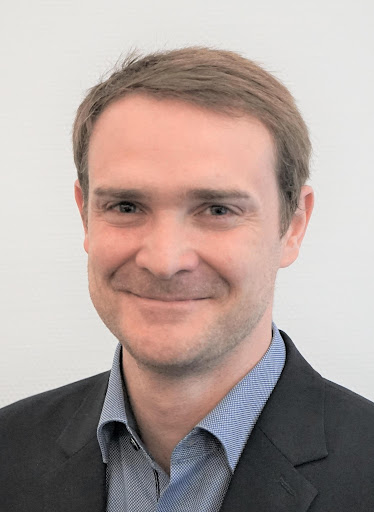
\includegraphics[width=2.5cm]{wick}}}}
    \end{picture}
}